\documentclass[11pt,fleqn]{article} % Default font size and left-justified equations

%\usepackage{standalone}

\usepackage{comment}
\begin{comment}
Modification History:
  180803 David Shifflett
    Fixed 'git clone https' syntax, added 'git clone git@' example
\end{comment}

\usepackage{todonotes}
\usepackage{color}
\usepackage{paralist}
% use \todo{note} OR \missingfigure{Add my picture here}

\usepackage[top=3cm,bottom=3cm,left=3.2cm,right=3.2cm,headsep=10pt,a4paper]{geometry} % Page margins
\usepackage{xcolor} % Required for specifying colors by name
\definecolor{ocre}{RGB}{243,102,25} % Define the orange color used for highlighting throughout the book


% Font Settings


% SLG commented out


% \usepackage{avant} % Use the Avantgarde font for headings
%\usepackage{times} % Use the Times font for headings
% \usepackage{microtype} %Slightly tweak font spacing for aesthetics
% \usepackage{mathptmx} % Use the Adobe Times Roman as the default text font together with math symbols from the Sym­bol, Chancery and Com­puter Modern fonts


%  \usepackage[scaled=0.90]{couriers} %What is this used for?




% SLG commented out
% \def\thereforesymbol{
% \leavevmode
% \lower0.1ex\hbox{$\cdot$}
% \kern-0.2em\raise0.7ex\hbox{$\cdot$}
% \kern-0.2em\lower0.2ex\hbox{$\cdot$}
% \thinspace}


% \usepackage{CJKutf8}
%For cyrillic characters  (do we have any?)


% slg commented this out:
% \usepackage[OT2,T1]{fontenc}
% \DeclareSymbolFont{cyrletters}{OT2}{wncyr}{m}{n}
% \DeclareMathSymbol{\Sha}{\mathalpha}{cyrletters}{"58}


\usepackage[T1]{fontenc}
\usepackage[section]{placeins}

% slg commented these out:
% \usepackage{amssymb}
 \usepackage{fancyvrb}
%  \usepackage{color}




%define a verbatim text for bold user input
\newcommand\verbbf[1]{\textbf{$\blacksquare$ #1}}
%define a verbatim text without box in front
\newcommand\verbbnbf{\textbf}


\PassOptionsToPackage{hyphens}{url}


\usepackage[pdftitle={Montery Phoenix Gryphon Toolset Users Manual},
              pdfauthor={Bruce Allen},
              pdfkeywords={monterey pheonix, system process modeler, trace generator}]{hyperref}
\makeatletter
\g@addto@macro{\UrlBreaks}{\UrlOrds}
\makeatother
% \usepackage{microtype} % Slightly tweak font spacing for aesthetics
%\usepackage[utf8]{inputenc} % Required for including letters with accents
\usepackage[T1]{fontenc} % Use 8-bit encoding that has 256 glyphs




%\usepackage[a4paper,pdftex]{geometry}                                                                                % A4paper margins
\setlength{\oddsidemargin}{5mm}                                                                                                % Remove 'twosided' indentation
\setlength{\evensidemargin}{5mm}


\usepackage[english]{babel}
%\usepackage[protrusion=true,expansion=true]{microtype}        
\usepackage{amsmath,amsfonts,amsthm,amssymb}
\usepackage{graphicx}


\usepackage{tabularx}


% Simson commented this out:
%use autoref or Autoref for lowercase or uppercase beginning of references
\usepackage{catoptions}
\makeatletter
\def\figureautorefname{figure}
\def\tableautorefname{table}
\def\Autoref#1{%
  \begingroup
  \edef\reserved@a{\cpttrimspaces{#1}}%
  \ifcsndefTF{r@#1}{%
    \xaftercsname{\expandafter\testreftype\@fourthoffive}
      {r@\reserved@a}.\\{#1}%
  }{%
    \ref{#1}%
  }%
  \endgroup
}
\def\testreftype#1.#2\\#3{%
  \ifcsndefTF{#1autorefname}{%
    \def\reserved@a##1##2\@nil{%
      \uppercase{\def\ref@name{##1}}%
      \csn@edef{#1autorefname}{\ref@name##2}%
      \autoref{#3}%
    }%
    \reserved@a#1\@nil
  }{%
    \autoref{#3}%
  }%
}
\makeatother


\usepackage{amsmath}


\usepackage{booktabs}


% slg commented out:
% \usepackage{makecell}


\usepackage{color}
\usepackage{graphicx}
%\usepackage {hyperref}
\usepackage{listings}
\lstset{
    literate={~} {$\sim$}{1}
}
\usepackage{xspace}


% slg commented out:
\usepackage[toc, page]{appendix}
\usepackage[labelfont=bf]{caption}
%http://tex.stackexchange.com/questions/27663/using- bold-italic-text-inside-listings


% slg commented out:
% \usepackage{multirow} %for multirow tables




\newcommand{\HRule}{\rule{\linewidth}{0.5mm}}
\usepackage{fancyhdr}


\usepackage{array}



\setcounter{secnumdepth}{5}
\setcounter{tocdepth}{5}

%\usepackage{arabtex}

\usepackage{verbatim}

\raggedbottom

\begin{document}

%define macros for commonly used terms that require special formatting
\newcommand \mpgt {\textit{MP Gryphon Toolset}\xspace}
\newcommand \ggui {\textit{MP Gryphon GUI}\xspace}
\newcommand \gtg {\textit{MP Gryphon Trace Generator}\xspace}
\newcommand \mphoenix {\textit{Monterey Phoenix}\xspace}

\hypersetup{%
    pdfborder = {0 0 0}
}

\lstdefinestyle{customfile}{
basicstyle=\footnotesize\ttfamily, frame=single, float=htpb}

\begin{titlepage}





% LaTeX Template: Titlepage
% This is a title page template which be used for both articles and reports.
%
% Copyright: http://www.howtotex.com/
% Date: April 2011
% ------------------------------------------------------------------------------

% -------------------------------------------------------------------------------
% Preamble
% -------------------------------------------------------------------------------
%\documentclass[paper=a4, fontsize=11pt,twoside]{scrartcl}		% KOMA article


% ------------------------------------------------------------------------------
% Definitions (do not change this)
% ------------------------------------------------------------------------------
\newcommand{\TRule}[1]{\rule{\linewidth}{#1}} 	% Horizontal rule

\makeatletter							% Title
\def\printtitle{%						
    {\centering \@title\par}}
\makeatother									

\makeatletter							% Author
\def\printauthor{%					
    {\centering \large \@author}}				
\makeatother							

% ------------------------------------------------------------------------------
% Metadata (Change this)
% ------------------------------------------------------------------------------
\title{	\LARGE \textsc{\mpgt} 	% Subtitle of the document
		 	\\[1.0cm]													% 2cm spacing
			\TRule{0.5pt} \\										% Upper rule
			\LARGE \textbf{\uppercase{Users Manual}}	% Title
			\TRule{2pt} \\ [0.5cm]								% Lower rule + 0.5cm spacing
			%\small \textit{Quickstart Guide Included}\\
			\normalsize \today									% Todays date
		}
\author{
		Authored by: \\
		Bruce D. Allen\\
}

% ------------------------------------------------------------------------------
% Maketitle
% ------------------------------------------------------------------------------
\thispagestyle{empty}				% Remove page numbering on this page

\printtitle									% Print the title data as defined above
  	\vfill
\printauthor								% Print the author data as defined above














\end{titlepage}


\pagenumbering{roman}
\setlength{\parindent}{0pt} %remove indenting from whole document
\newpage
\thispagestyle{empty}
\mbox{}
\newpage

\tableofcontents
\newpage
\pagenumbering{arabic}
\newpage

\section{Introduction}
\label{intro}
\subsection {Overview}
The \mpgt supports \mphoenix users with tools for building MP Code and generating trace graphs calculated from MP code.
The \mpgt consists of the \ggui and the \gtg.\\
\begin{compactitem}
\item The \ggui tool is the graphical interface tool for editing MP Code and for running the \gtg engine to view generated traces.
\item The \gtg tool compiles MP Code into traces that the \ggui can read and graph.\\
\end{compactitem}

\subsection{Compatibility}
\ggui Version 0.4.3 is compatible with \mphoenix Version 4 and the \gtg Version 4.\\

The \gtg Version 4 is currently compatible with Linux flavors and with older Macintosh systems.  The \gtg is currently not compatible with Windows systems because C++ compilation is not worked out and is not compatible with default Macintosh systems High Sierra 10.13.4 and later because 32-bit support is discontinued.
\section{Installing the \mpgt}
You will need the \ggui and the \gtg.
%  What you need depends on whether you are running Mac/Linux or Windows and the installation approach you choose.
For now, for Mac/Linux: clone \mpgt source code directly from their Git repositories.  For example to install under directory \verb+gits_mp+ in your home directory, type the following:
\begin{Verbatim}[commandchars=\\\{\}]
\verbbf{mkdir ~/gits_mp}
\verbbf{cd ~/gits_mp}
\verbbf{git clone https://gitlab.nps.edu/monterey-phoenix/trace-generator.git}
\verbbf{git clone https://gitlab.nps.edu/monterey-phoenix/user-interfaces/gryphon.git}
\end{Verbatim}

or if you prefer using the git protocol:
\begin{Verbatim}[commandchars=\\\{\}]
\verbbf{mkdir ~/gits_mp}
\verbbf{cd ~/gits_mp}
\verbbf{git clone git@gitlab.nps.edu:monterey-phoenix/trace-generator.git}
\verbbf{git clone git@gitlab.nps.edu:monterey-phoenix/user-interfaces/gryphon.git}
\end{Verbatim}

If using the git protocol, you will need to upload your public RSA Key as described at \url{https://gitlab.nps.edu/help/ssh/README.md}.\\

\subsection{Installing Python 3}
Install Python3 if it is not already present. To see if Python3 is already installed, you may type the following at a command prompt and verify that Python Version 3 is present:
\begin{compactitem}
%\item Windows:
%\begin{Verbatim}[commandchars=\\\{\}]
%\verbbf{python --version}
%\end{Verbatim}
\item Mac/Linux:
\begin{Verbatim}[commandchars=\\\{\}]
\verbbf{python3 --version}
\end{Verbatim}
\end{compactitem}
If not already present, you may download and install Python3 for your system from \url{https://www.python.org/download/releases/3.0}.\\
%If installing on Windows, you must check the ``Add Python to PATH'' checkbox when installing Python or you will get an error indicating that Python is not recognized.\\

Linux users may prefer to install Python 3 using their package manager, for example Fedora users might type:
\begin{Verbatim}[commandchars=\\\{\}]
\verbbf{sudo dnf install python3+}
\end{Verbatim}

\subsection{Installing PyQt5}
The \ggui requires PyQt5.
Please type the following at a command prompt to install PyQt5:
\begin{compactitem}
%\item Windows:
%\begin{Verbatim}[commandchars=\\\{\}]
%\verbbf{python -m pip install PyQt5}
%\end{Verbatim}
\item Mac/Linux:
\begin{Verbatim}[commandchars=\\\{\}]
\verbbf{python3 -m pip install PyQt5}
\end{Verbatim}
\end{compactitem}

\subsection{Building the \gtg}
If you installed on Mac/Linux using the repositories then the \gtg must be built.
First, please install requisites needed for running \verb+make+.
Mac users may be asked to install Command line developer tools, which are required.  Linux users need to install 32-bit CLib and the csh shell. Syntax depends on Linux flavor.  A Fedora dnf example is to type:
\begin{Verbatim}[commandchars=\\\{\}]
\verbbf{sudo dnf install glibc-devel.i686}
\verbbf{sudo dnf install tcsh.x86_64}
\end{Verbatim}

An Ubuntu apt example is:
\begin{Verbatim}[commandchars=\\\{\}]
\verbbf{sudo apt install libc6-dev-i386}
\verbbf{sudo apt install csh}
\end{Verbatim}

Build the trace generator engine from a command window by typing:
\begin{Verbatim}[commandchars=\\\{\}]
\verbbf{cd ~/gits_mp/trace-generator/RIGAL/rigsc.446/src}
\verbbf{make}
\end{Verbatim}

%%% For zip or Windows installer:
%\subsubsection{Downloading and Running the \ggui}
%\begin{compactitem}
%\item Windows users:
%  \begin{compactenum}
%  \item Download the \ggui Windows Installer from the \mpgt Download page.
%  \item Click on the download and run the installer.
%  \item Start the \ggui tool by clicking on the \ggui tool icon.
%  \end{compactenum}
%\item Mac, Linux flavors, and Windows users: All users may install and run the \ggui \verb+.zip+ distribution as follows:
%  \begin{compactenum}
%  \item Download the \ggui \verb+.zip+ distribution from the \mpgt Download page.  For example you might download it to\\
%\verb+/Users/<yourname>/Downloads+.
%  \item Unzip the distribution.
%  \item From a command window, navigate to the \verb+MP_Gryphon_GUI/python/+ subdirectory, for example to path\\
%\verb+/Users/<yourname>/Downloads/MP_Gryphon_GUI_<latest version>/python+ and type:
%\begin{Verbatim}[commandchars=\\\{\}]
%\verbbf{./mp.py}
%\end{Verbatim}
%  \end{compactenum}
%\end{compactitem}
%

\section{Launching the \ggui}
For Mac/Linux users: from a command window, navigate to the directory containing the \ggui tool and run it by typing:
\begin{Verbatim}[commandchars=\\\{\}]
\verbbf{cd ~/gits_mp/gryphon/python}
\verbbf{./mp.py}
\end{Verbatim}

\subsection{Configuring the \ggui}
Once launched, the \ggui may be configured using its menu controls under \verb+Preferences+:
\begin{compactitem}
\item Several graph appearance options are available optimized for brightness, printing, a classic look, etc.\\
\end{compactitem}


\section{Working with the \ggui}
To write your own system models, a working knowledge of \mphoenix technology and MP Code syntax is required. Please visit \url{https://wiki.nps.edu/display/MP/Monterey+Phoenix+Home} for information about working with \mphoenix technology.

\section{\ggui User Interfaces}
%\subsection{Main Window}
This section describes user interfaces available to \ggui.
Here is an example screenshot of the \ggui main window:\\
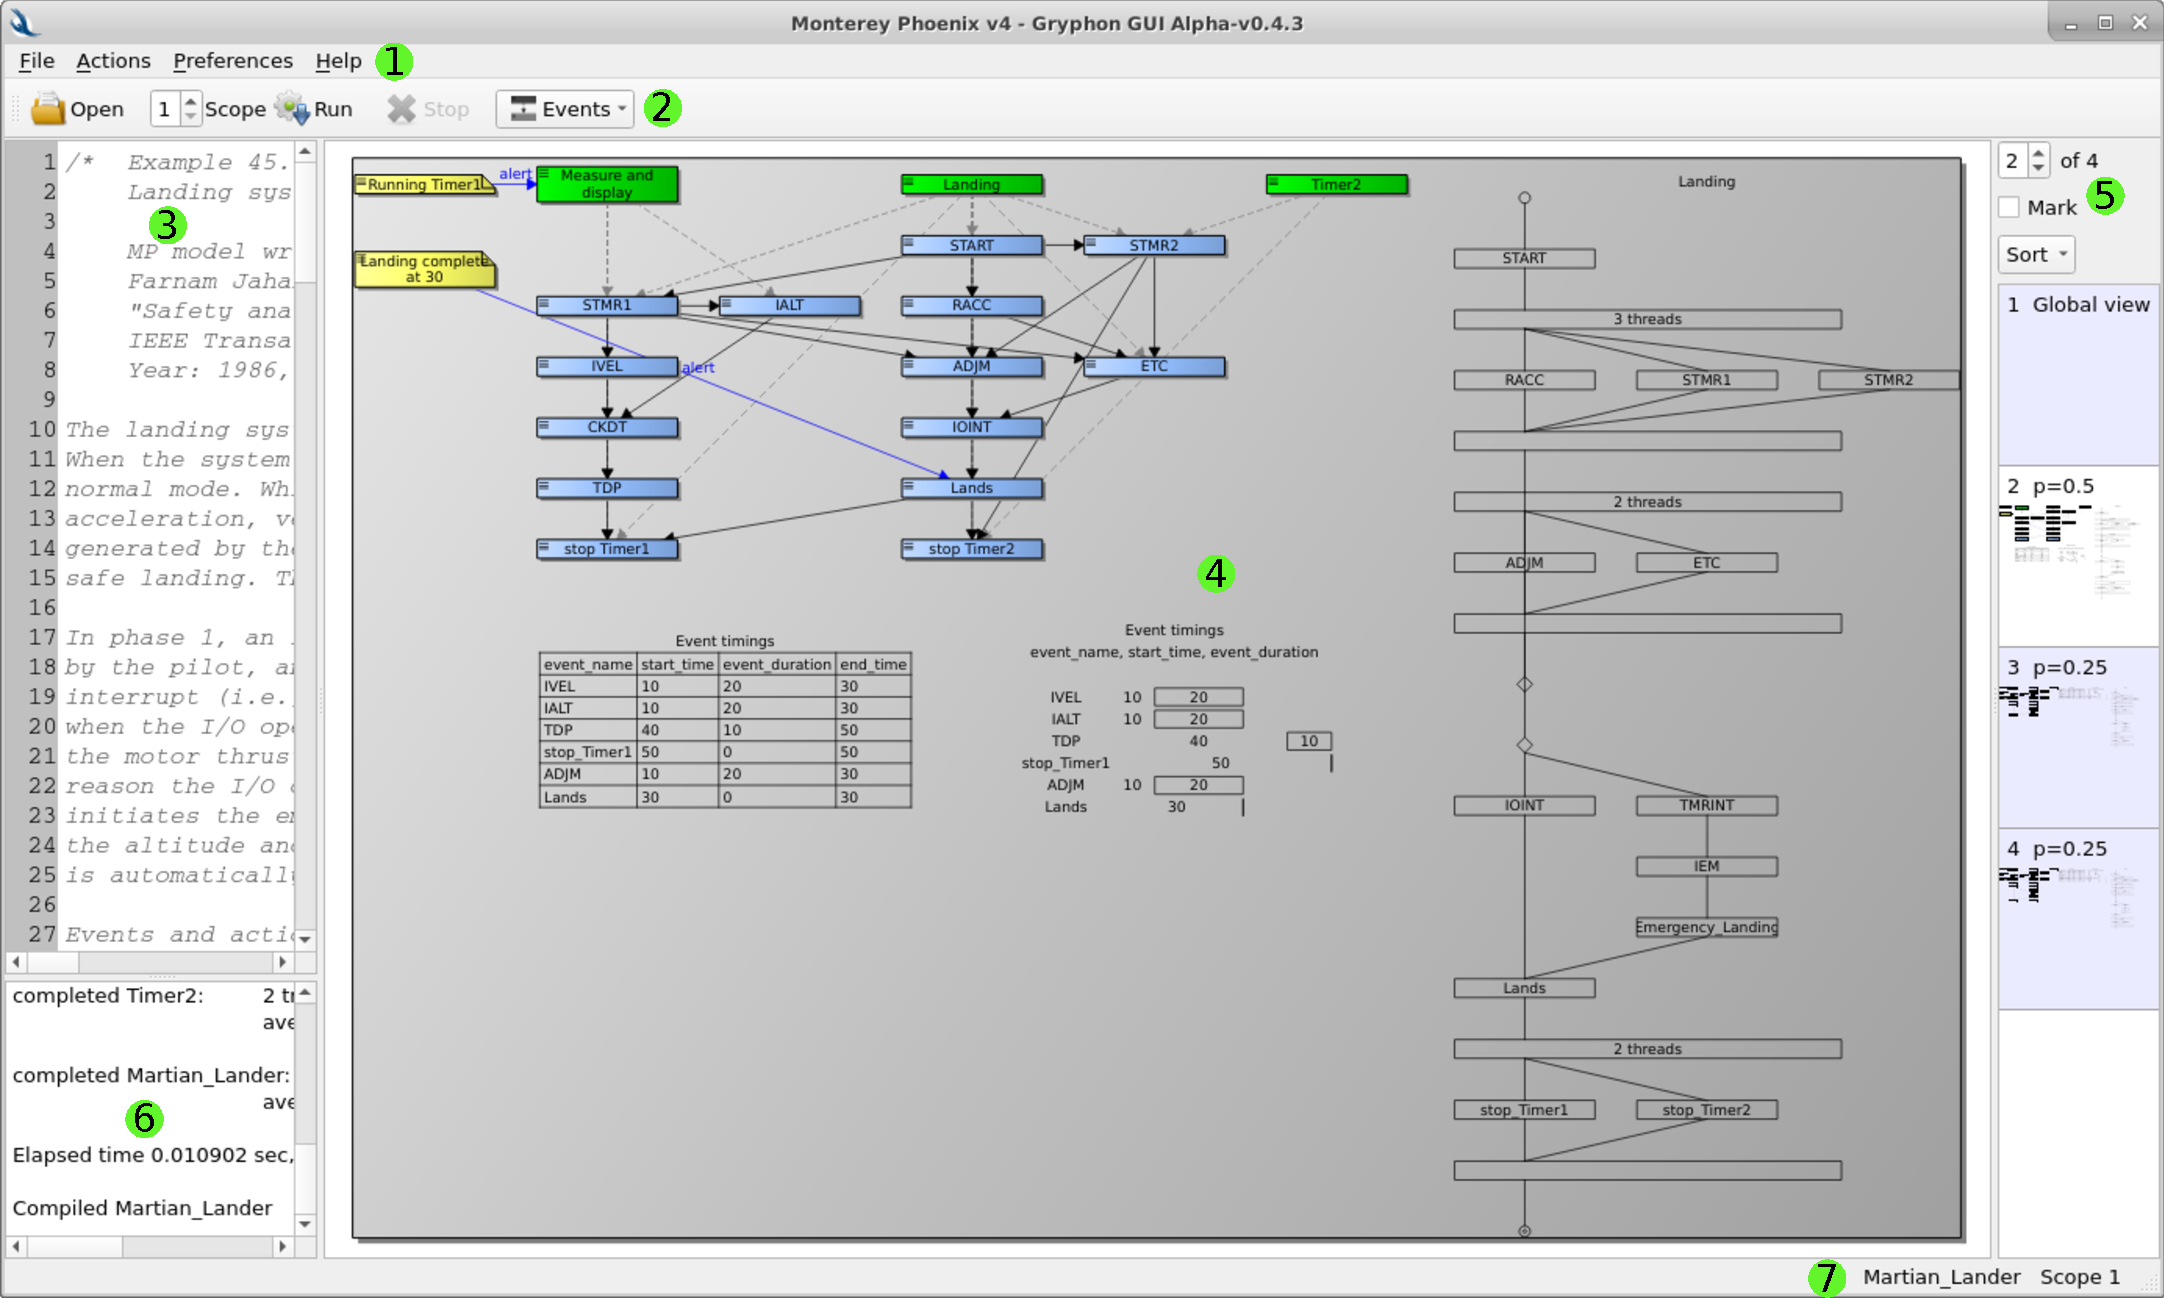
\includegraphics[scale=.4]{screenshots/main_window_ex45mod_sectioned}\\
The following parts are shown:
\begin{compactenum}
\item Menu controls
\item Toolbar shortcuts
\item MP Code editor
\item Main graph view
\item Navigation column
\item Log pane
\item Status
\end{compactenum}

\subsection{Menu Controls}
Menu controls include:
\begin{compactitem}
\item \textbf{File}
  \begin{compactitem}
  \item Open, save MP Code, open examples.
  \item Import and export projects as Gryphon .gry files.
  \item Export one or all graphs as .png files.
  \end{compactitem}
\item \textbf{Actions}
  \begin{compactitem}
  \item Run the trace generator engine.
  \item Clear the Log pane.
  \end{compactitem}
\item \textbf{Preferences}
  \begin{compactitem}
  \item Graph Settings: Set graph settings:
    \begin{compactitem}
    \item Bright - View with high color contrast.
    \item Print - View with colors that are more readable when printed.
    \item Classic - Use classic Firebird coloring.
    \item Custom - Set, save, share your own color scheme.
    \end{compactitem}
  \item Server: Set to connect to a \gtg Server or to use the \gtg locally.
  \end{compactitem}
\item \textbf{Help}
  \begin{compactitem}
  \item View help for the \mpgt.
  \item View information about \mpgt.
  \end{compactitem}
\end{compactitem}

\subsection{Toolbar shortcuts}
Trace generater controls are available in the toolbar.  This toolbar shows controls with Scope 1 selected:

\includegraphics[scale=.4]{screenshots/toolbar}.\\
Hover the cursor over controls to see tooltips. Controls include:
\begin{compactitem}
\item The ``Open MP Code File'' button (
\includegraphics[scale=.4]{screenshots/open_mp_code_file}) for opening a MP Code file.
\item The ``Scope'' selector
(
\includegraphics[scale=.4]{screenshots/scope_spinner})
for selecting the scope for trace generation.
\item The ``Run'' button (
\includegraphics[scale=.4]{screenshots/run})
for running the trace generator engine on the MP Code.
\item The ``Stop'' button (
\includegraphics[scale=.4]{screenshots/stop})
for aborting a trace generator run.
\item The ``Events'' button (
\includegraphics[scale=.4]{screenshots/events})
to open a menu for controlingcontrol how events are displayed:
  \begin{compactitem}
  \item Show Hidden Events.
  \item Collapse Root Events.
  \item Expand Root Events.
  \item Collapse Composite Events.
  \item Expand Composite Events.
  \item Hidden/Collapsed opacity (0\%, 25\%, 50\%, 75\%).
  \end{compactitem}
\end{compactitem}

\subsection{MP Code Editor Pane}
Manage MP Code using the MP Code editor pane:
\begin{compactitem}
\item Open, import, paste, or edit your MP Code.
\item Syntax highlighting identifies keywords, root events, composite events, etc.
\item Run the trace generator engine (
\includegraphics[scale=.4]{screenshots/run}) at the desired scope 
(
\includegraphics[scale=.4]{screenshots/scope_spinner})
to generate traces from your MP Code.
\end{compactitem}

\subsection{Main Graph View}
The main graph view displays the global view or trace currently selected in the navigation column.
You may adjust this view as follows:
\begin{compactitem}
\item Pan by dragging the mouse or moving the scrollbars.
\item Zoom by moving the mouse wheel or by pressing the \verb.+. or \verb+-+ keys. The zoom focal point is at the cursor.
\item Drag nodes to move them.
\item You may also adjust view settings using menu control \verb+Preferences | Graph Setti+ \verb+ngs | Custom...+.
\item Select a node's menu icon to collapse, expand, hide, or show that node.
\item Select an edge and then move its Bezier curve to move edges.
\end{compactitem}

\subsection{Navigation Column}
The navigation column contains the following:
\begin{compactitem}
\item The index of the current graph, in this example, 2: (
\includegraphics[scale=.4]{screenshots/navigation_index}). Select a different index using this control or via the graph list.
\item Whether traces are filtered by Mark, in this example, not filtered by mark: (
\includegraphics[scale=.4]{screenshots/filter_by_mark}).
\item Trace sort control menu (
\includegraphics[scale=.4]{screenshots/trace_sort}) containing controls for sorting by trace index, mark, probability, or size.
\item The graph list.  The first graph is the global view, or blank if there is none.  The remaining graph(s) identify the list of all possible traces given your MP Code and scope.\\

At the top of each graph is its graph index. For traces, the probability of that trace occurring is also displayed, where the sum of probabilities across all traces is 1.0.\\

Navigate the graph list as follows:
  \begin{compactitem}
  \item Scroll down to view all graphs.
  \item Click on a graph (global view or trace) to select it in the main graph view pane.
  \item Once clicked on, use the up and down keyboard shortcut to navigate up and down through the graphs.
  \end{compactitem}
\end{compactitem}

\subsection{Log Pane}
The log pane provides a log of actions taken and of trace generator output. It is available for reference. You may clear it using menu control \verb+File | Actions | Clear MP Code Log+.

\subsection{Status}
Status describes information about the currently loaded trace generation view.
In this example,

\includegraphics[scale=.4]{screenshots/example_status}:
\begin{compactitem}
\item \verb+Martian_Lander+ is the name of the schema as defined in the MP Code.
\item \verb+Scope 1+ indicates that the trace generator engine was run for the MP Code at scope level 1.
\end{compactitem}

\subsection{Keyboard Shortcuts}
\subsubsection{Graph Window Shortcuts}
\begin{compactitem}
\item CTRL + Click on event (Command + Click on Mac): Toggle select or unselect individual events.
\item SHIFT + Click on event: Select event and all events below it bound by IN relation.
\item Click empty space: Unselect all events.
\item Click on empty space and drag: Pan the view.
\item SHIFT + Click empty space and drag: Select events in range.
\item CTRL + A (Command + A on Mac): Select all events.
\item Keyboard arrow keys: Pan the view.
\item + and - keys: Zoom in and out.
\item Click menu tab: Open menu for an event.
\item Right-click event: Open menu for an event.
\item H: Toggle hide/unhide selected event(s).
\item C: Toggle collapse/uncollapse selected Root and Composite event(s). Results may be unexpected if multiple events are selected.
\end{compactitem}

\subsubsection{Code Window Shortcuts}
\begin{compactitem}
\item Click word to highlight word.
\item Click or Navigate to parenthesis to find its mate.
\item CTRL + Spacebar or type first three letters: Show auto-complete hints for existing events or keywords.
\end{compactitem}

\subsubsection{Graph List Shortcuts}
\begin{compactitem}
\item Up and down arrows: Select previous or next graph.
\end{compactitem}

\section{Examples}
Please obtain, install, and start the \ggui graphical interface per installation instructions, above.
\subsection{Load and run MP Code Example 1}
In this example we open and run MP Code example 1 at Scope 2, select and adjust trace 2, and save the view as a \verb+.png+ image file.

\begin{compactenum}
\item Under menu control \verb+File | Open MP Code Example+ select example\\
\verb+Example_1_simple_message_flow.mp+.
The MP Code listing will show up in the code editor pane.
\item Set the scope to 2 by adjusting the Scope spinner trace generator control.
\item Run the trace generator engine by pressing the run icon
(
\includegraphics[scale=.4]{screenshots/run}).
Four graphs will be generated, a global view graph and three traces. All four graphs will be visble in the graph navigation list. The global view, if there was one, would be visible in the main graph view pane.
\item Select the fourth graph in the list. It will be drawn in the main graph view.
\item Move some nodes as desired by dragging them with the cursor.
\item Export the selected graph to a \verb+.png+ file using menu \verb+File | Export Graph...+.
\item If you would like to print your exported graphs, you may wish to select menu control \verb+Preferences | Graph Settings | Contrast+ for higher contrast for printing before exporting them. Or select menu control \verb+Preferences | Graph Settings | Custom...+ to configure your own graph view scheme. Then use menu \verb+File | Export All Graphs...+.
\end{compactenum}

\section{Reporting Bugs}
Please report any bugs encountered during operation of the \mpgt.  To assist in diagnosing your bug, please include the following informtion:
\begin{compactitem}
\item The \verb+.mp+ code, Scope number, and the graph index selected when the error occurred.
\item The steps taken that can be used to recreate the error.
\item The version of the \ggui tool used.
\item The Operating System you used.
\end{compactitem}

\section{Post-processing Analysis}
The \ggui tool exports graph data in JSON Graph format (JGF).
This output may be used during post-processing analysis of graph data or for input to third party tools which can accept JGF data as input.
The JGF standard defines names for \verb+graph+, \verb+node+, and \verb+edge+ fields. The \ggui tool extends these fields by including additional information such as graph positioning, the trace \verb+mark+ field, Cubic Bezier edge points for curved edges, and whether nodes are hidden or collapsed.
For more information on JGF please see \url{http://jsongraphformat.info}. For syntax of JSON data exported by the \ggui tool, please use the export command to create your own JSON \verb+.gry+ file and use that as a reference.

\end{document}
